
\documentclass[article]{jss}

%%%%%%%%%%%%%%%%%%%%%%%%%%%%%%
%% declarations for jss.cls %%%%%%%%%%%%%%%%%%%%%%%%%%%%%%%%%%%%%%%%%%
%%%%%%%%%%%%%%%%%%%%%%%%%%%%%%

%% almost as usual
\author{Andreas Hill \\ETH Z\"urich \And 
        Alexander Massey}
\title{The \proglang{R} Package \pkg{forestinventory}: Design-Based Global and Small Area Estimations for Multiphase Forest Inventories}

%% for pretty printing and a nice hypersummary also set:
\Plainauthor{Andreas Hill, Alexander Massey} %% comma-separated
\Plaintitle{A Capitalized Title: Something about a Package foo} %% without formatting
\Shorttitle{\pkg{forestinventory}: Design-Based Global and Small Area Estimations} %% a short title (if necessary)

%% an abstract and keywords
\Abstract{
Forest inventories provide reliable and evidence based information to assess the state and development of forests over time. The information is collected at discrete sample locations distributed over the forest area by means of statistical sampling methods. This sample is then used to provide estimates of a target variable for a given spatial unit. Due to the high costs of the terrestrial campaigns, there is a need for alternative methods that can provide a) the same estimation precision at lower costs or b) higher estimation precision at identical costs. With respect to this objective, the application of double- and triple-sampling regression estimators (so-called \textit{multiphase} forest inventory methods) has proved to be efficient. The core concept of multiphase methods is to combine the terrestrial sample with a much larger sample of target variable \textit{predictions} based on \textit{auxiliary information} that is available in high quantity and low costs. Whereas these methods have been successfully applied in practice, the availability of repective open-source software has been rare up to non-existent. The \proglang{R} package \pkg{forestinventory} provides a comprehensive set of global and small area regression estimators for multiphase forest inventories under simple and cluster sampling. The implemented methods have been demonstrated in various scientific studies covering small to large scale forest inventories, and can be used for double- and triple sampling for stratification, regression and regression within strata. This article provides a bridge from the mathematical summary of the estimators to their implementation and application in \proglang{R}.}

\Keywords{forest inventory, design-based, infinite population approach, two and three phase sampling, regression estimators, small area estimation}
\Plainkeywords{forest inventory, design-based, infinite population approach, two and three phase sampling, regression estimators, small area estimation}

%% publication information
%% NOTE: Typically, this can be left commented and will be filled out by the technical editor
%% \Volume{50}
%% \Issue{9}
%% \Month{June}
%% \Year{2012}
%% \Submitdate{2012-06-04}
%% \Acceptdate{2012-06-04}

%% The address of (at least) one author should be given
%% in the following format:
\Address{
  Andreas Hill\\
  Department of Environmental Systems Science\\
  Chair of Landuse Engineering\\
  ETH Z\"urich\\
  Universit\"atstrasse 16\\
  8092 Z\"urich, Switzerland\\
  E-mail: \email{andreas.hill@usys.ethz.ch}\\
  Telephone: +41/44/632 32 36\\
  URL: \url{http://www.lue.ethz.ch/people/hilla}
  
  Alexander Massey\\
  Department of Environmental Systems Science\\
  Chair of Landuse Engineering\\
  ETH Z\"urich\\
  Universit\"atstrasse 16\\
  8092 Z\"urich, Switzerland\\
  E-mail: \email{afmass@gmail.com}\\}
}


%% for those who use Sweave please include the following line (with % symbols):

%% need no \usepackage{Sweave.sty}

%% end of declarations %%%%%%%%%%%%%%%%%%%%%%%%%%%%%%%%%%%%%%%%%%%%%%%


%------------------------------------------------------------------------------------------------%
% -------------------------------------- Tex Settings ------------------------------------------ %

% used packages
\usepackage{amsmath}
\usepackage{amsfonts}
\usepackage{mathptmx} 
\usepackage{latexsym}
\usepackage{a4}
\usepackage{graphicx}
\usepackage{epsfig}
\usepackage{caption}
\usepackage{subcaption}
\usepackage{flafter}
\usepackage{bm}
\usepackage{setspace}
\usepackage{lineno}
\usepackage{natbib}
\usepackage{geometry}
 \geometry{
 a4paper,
 left=28mm,
 bottom=28mm
 }
\usepackage[labelfont=bf]{caption}
\usepackage[font=footnotesize]{caption}
\usepackage[font=footnotesize]{subcaption}

% new commands
\newcommand{\bwi}{BWI3}
\newcommand{\LF}{\ensuremath{\lambda(F)}}
\newcommand{\LFC}{\ensuremath{\lambda^2(F)}}
\newcommand{\EX}{\mathbb{E}}
\newcommand{\PR}{\mathbb{P}}
\newcommand{\var}{\mathbb{V}}
\newcommand{\COV}{\mathbb{COV}}
\newcommand{\MAV}{\mathbb{MAV}}
\newcommand{\MRAV}{\mathbb{MRAV}}
\newcommand{\POP}{\mathcal{P}}
\newcommand{\SAMP}{\mathcal{S}}
\newcommand{\RE}{\mathbb{RE}}
\newcommand{\PLAN}{\Re^2}
\newcommand{\SUR}{\mathbb{S}}
\newcommand{\ING}{\mathbb{I}}
\newcommand{\DEP}{\mathbb{D}}

%\setlength{\parindent}{1em}

%------------------------------------------------------------------------------------------------%
% -------------------------------------- Main Document------------------------------------------ %

\begin{document}


%------------------------------------------------------------------------------------------------%
% -------------------------------------- R Settings -------------------------------------------- %


% set global options for R-output:


%------------------------------------------------------------------------------------------------%
% ---------------------------------- Introduction ---------------------------------------------- %

% !Rnw root = JStatSoft_forestinventory_master.Rnw

\section{Introdution}
\label{sec:intro}

In many countries, forest inventories have become an integral instrument to judge the current state as well as the development of forests within reoccurring time periods. They provide quantitative information when it comes to define management actions and to adapt forest management strategies according to guidelines on national- and international level. Whereas the most straightforward approach of collecting the required information would be a full census of all trees within the forest area of interest, this remains only feasible for spatially small areas and is even then scarcely done in practice due to time- and cost restrictions. For this reason, forest inventories gather their information of interest by means of statistical sampling methods, i.e. information is gathered only at discrete sample locations (\textit{sample plots}) in the forest in the framework of a \textit{terrestrial inventory}. This sample is then used to provide estimations of a target variable for a given spatial unit, and there is a broad range of concepts and methods regarding the choice of the sample design and respective estimators \citep{gregoire2007, kohl2006, schreuder1993, mandallaz2008}. The information of terrestrial samples is assumed to be very precise, and increasing the precision of the estimates could primarily be achieved by increasing the terrestrial sample size. However, since collecting the terrestrial information is very time consuming and expensive, the number of terrestrial samples is usually limited. Whereas in national inventories the terrestrial sample size is still sufficient to provide high estimation accuracies on the national scale, small sample sizes on smaller spatial scales such as forest management units often cause high estimation errors that hamper using the inventory information.\par

Developments in recent years thus showed an increasing need for alternative inventory methods that can maintain the same estimation precision at lower costs, or achieve higher estimation precision at identical costs \citep{vonluepke2013}. A method which has become particularly attractive is so called \textit{multiphase sampling}. The core concept is to enlarge the sample size in order to gain higher estimation precision \textit{without} enlarging the terrestrial sample size. This is done by using predictions of the terrestrial target variable at additional sample locations where the terrestrial information has not been gathered. These predictions are produced by regression models that use explanatory variables derived from auxiliary data, commonly in the form of spatially exhaustive remote sensing data in the inventory area. Regression estimators using this concept can consider either \textit{one} additional sample of auxiliary information (two-phase or double-sampling) or \textit{two} additional samples of auxiliary information available in different sample sizes (three-phase or triple-sampling) \citep{gregoire2007, saborowski2010, mandallaz2013a, mandallaz2013c, vonLüpke2012}. Their application to existing forest inventory systems have already showed their efficiency in terms of cost reduction and gain in estimation precision \citep{breidenbach2012, vonLuebke2014, mandallaz2013b, magnussen2014, massey2014a}.\par

% section:briefly give a review of existing R-packages for forest inventories (not much around) and 
Despite these promising developments, a standard application of two and three-phase sampling methods in forest practice has been hampered by a lack of available software. One exception is the \proglang{R} package \pkg{JoSAE} by \citet{josae2015} that provides the GREG \citep{sarndal2003} and EBLUP \citep{battese1988} two-phase small area estimator for simple sampling derived under the finite population approach. However, a more comprehensive software package covering a larger variety of sampling designs and estimators applicable to forest inventories has up to now been missing. Our motivation has been to addressed this lack by the \proglang{R} package \pkg{forestinventory}. The package provides global and small area estimators for two-phase and three-phase forest inventories under simple and cluster sampling, which have been developed under the infinite population approach by Daniel Mandallaz at ETH Zurich between 2008 and 2017. The implemented methods have been demonstrated by case studies in Switzerland \citep{massey2014a, massey2015b, mandallaz2013b} and Germany \citep{hill2017a}. The package comprises two- and three phase sampling regression estimators for global and small area estimations under simple and cluster sampling design and thus cover 32 inventory scenarios in total. The estimators can be used for stratification, regression and regression within strata \citep{massey2015}. The long-term objective of \pkg{forestinventory} is to make the broad range of estimators available to a large user community and to facilitate their application in science as well as operational forest management.

The particular objective of this article is a) to establish the link between the mathematical description of the estimators and their implementation in our package, b) to illustrate their application by the respective functions in our package to real-world inventory scenarios and c) to highlight special cases, i.e. rare inventory scenarios, and demonstrate how the package-functions deal with such situations (including error-checking functions and data adjustments).



% what is the motivation of the package: - to make the broad range of Mandallaz-estimators
%              available to a large user community, to facilitate their application in science as well as 
%              operational forest management (why is this important? --> because the methods have demonstrate
%              the potential of considerably increasing the estimation precision)
% 4th section: whats the purpose of the paper? --> the objective of the paper is to 
%             a) establish the link between the mathematical description of the estimators (given in Mandallaz ...) 
%                and their implementation in our package
%             b) illustrate the application of the various estimators by the respsective functions in our package 
%                to real-world inventory scenarios
%             c) highlight 'special cases' , i.e. rare inventory scenarios, and demonstrate how the package-functions
%                deal with such situations (error-checking functions and data-adjustments)



% NOTES:
% --> take parts of the old introduction version of the diploma-thesis!

% NOTES:
% 1st section: - general introduction to forest inventories --> model-'supported' inventories --> 
%                model-dependent vs. design-based
% 2nd section: + (more R-specific): what's already there? --> mention sampling / inventory packages
%                 and seperate them from our package (focus, applied areas, approach)
%              + important reasoning for our package: we are the first that implemented and provide 
%                a large range of design-based estimators
% 3rd section: what is the motivation of the package: - to make the broad range of Mandallaz-estimators
%              available to a large user community, to facilitate their application in science as well as 
%              operational forest management (why is this important? --> because the methods have demonstrate
%              the potential of considerably increasing the estimation precision)
% 4th section: whats the purpose of the paper? --> the objective of the paper is to 
%             a) establish the link between the mathematical description of the estimators (given in Mandallaz ...) 
%                and their implementation in our package
%             b) illustrate the application of the various estimators by the respsective functions in our package 
%                to real-world inventory scenarios
%             c) highlight 'special cases' , i.e. rare inventory scenarios, and demonstrate how the package-functions
%                deal with such situations (error-checking functions and data-adjustments)

% Idee: Reine Theory und Applikation NICHT stark trennen --> Jeweils für jeden Schätzer die nötigsten Formeln geben 
%       (Punktschätzung und g-weight und external variance, wenn nötig noch zusätzliche Infos wie Dummy Variable)
%      WICHITG: Davor muss das generelle Konzept kommen (Entscheidungsbaum und konzeptionelle Erklärung (z.B.: was heisst
%               "exhaustive" usw.) --> auf der Graphik dann ansetzen
%
% evtl auch noch die Art von Graphik für den Aufbau einer 2- und 3-phaisgen Inventurs (wie in den Präsentationen)

% Explain the problem that leads to sae estimations (in generell and in forestry)
%
%




































% NOTES:
% --> take parts of the old introduction version of the diploma-thesis!

% NOTES:
% 1st section: - general introduction to forest inventories --> model-'supported' inventories --> 
%                model-dependent vs. design-based
% 2nd section: + (more R-specific): what's already there? --> mention sampling / inventory packages
%                 and seperate them from our package (focus, applied areas, approach)
%              + important reasoning for our package: we are the first that implemented and provide 
%                a large range of design-based estimators
% 3rd section: what is the motivation of the package: - to make the broad range of Mandallaz-estimators
%              available to a large user community, to facilitate their application in science as well as 
%              operational forest management (why is this important? --> because the methods have demonstrate
%              the potential of considerably increasing the estimation precision)
% 4th section: whats the purpose of the paper? --> the objective of the paper is to 
%             a) establish the link between the mathematical description of the estimators (given in Mandallaz ...) 
%                and their implementation in our package
%             b) illustrate the application of the various estimators by the respsective functions in our package 
%                to real-world inventory scenarios
%             c) highlight 'special cases' , i.e. rare inventory scenarios, and demonstrate how the package-functions
%                deal with such situations (error-checking functions and data-adjustments)

% Idee: Reine Theory und Applikation NICHT stark trennen --> Jeweils für jeden Schätzer die nötigsten Formeln geben 
%       (Punktschätzung und g-weight und external variance, wenn nötig noch zusätzliche Infos wie Dummy Variable)
%      WICHITG: Davor muss das generelle Konzept kommen (Entscheidungsbaum und konzeptionelle Erklärung (z.B.: was heisst
%               "exhaustive" usw.) --> auf der Graphik dann ansetzen
%
% evtl auch noch die Art von Graphik für den Aufbau einer 2- und 3-phaisgen Inventurs (wie in den Präsentationen)


%------------------------------------------------------------------------------------------------%
% --------------------------- Structure of the Package ----------------------------------------- %

% !Rnw root = JStatSoft_forestinventory_master.Rnw

%\section{Structure of the Package}
\section{Methods and Structure of the Package}
\label{sec:str_and_mod}


%Here comes the general structure of the package, or at least of the two and three-phase functions

\subsection{Two-Phase Sampling}

The two-phase or double-sampling estimators use inventory information from \textbf{two} nested samples which are commonly reffered to as \textit{phases} (figure \ref{fig:concmphase_and_sae_a}). The first phase $s_1$ comprises $n_1$ sample locations that provide a set of explanatory variables described by the column vector $\pmb{Z}(x)\in{\Re^{p}}$ at each point $x \in s_1$. These explanatory variables are derived from auxiliary information that is available in high quantity within the forest area $F$. The second phase $s_2$ constitutes the terrestrial inventory conducted at $n_2$ subsamples of the large phase $s_1$ and provides the value of the target variable, i.e. the local density $Y(x)$ such as the timber volume density per hectare. The set of explanatory variables at each sample location $x \in s_1$ is now transformed into a prediction $\hat{Y}(x)$ of $Y(x)$ by the application of an oridinary least square (OLS) regression model. In the \proglang{R} package \pkg{forestinventory}, estimators for two-phase sampling can be applied by the \code{twophase}-function. Their implementation and application is described in detail in section \ref{sec:globest_and_appl} and \ref{sec:saeest_and_appl}.


\subsection{Three-Phase Sampling}

The three-phase or triple-sampling estimators extend the principle of two-phase sampling and use inventory information from \textbf{three} nested samples (\textit{phases}). The basic assumption is that auxiliary information is available in two different sample sizes.




A first phase of auxiliary information (e.g. taken from remote sensing data) is used to generate model predictions based on multiple linear regression using the method of ordinary least squares. A subsample of the first phase comprises a second phase which contains further auxiliary information that produces another set of model predictions. A further subsample produces a third final phase based on terrestrial observations (i.e. the local densities of the ground truth) and is used to correct for bias in the design-based sense. The estimation method is available for simple and cluster sampling and includes the special case where the first phase is based on an exhaustive sample (i.e. a census). Small-area applications are supported for synthetic estimation as well as two varieties of bias-corrected estimators: the traditional small-area estimator and an asymptotically equivalent version derived under Mandallaz's extended model approach.


Explain three phase sampling, giving refrences to existing literature and studies


\begin{figure}[htb]
	\begin{subfigure}[t]{0.5\textwidth} 
		\centering
    \resizebox{1.1\hsize}{!}{\includegraphics{fig/multiphase_graphic.eps}}%
		\caption{} \label{fig:concmphase_and_sae_a}
		\end{subfigure}
	\begin{subfigure}[t]{0.5\textwidth} 
		\centering
   \resizebox{0.85\hsize}{!}{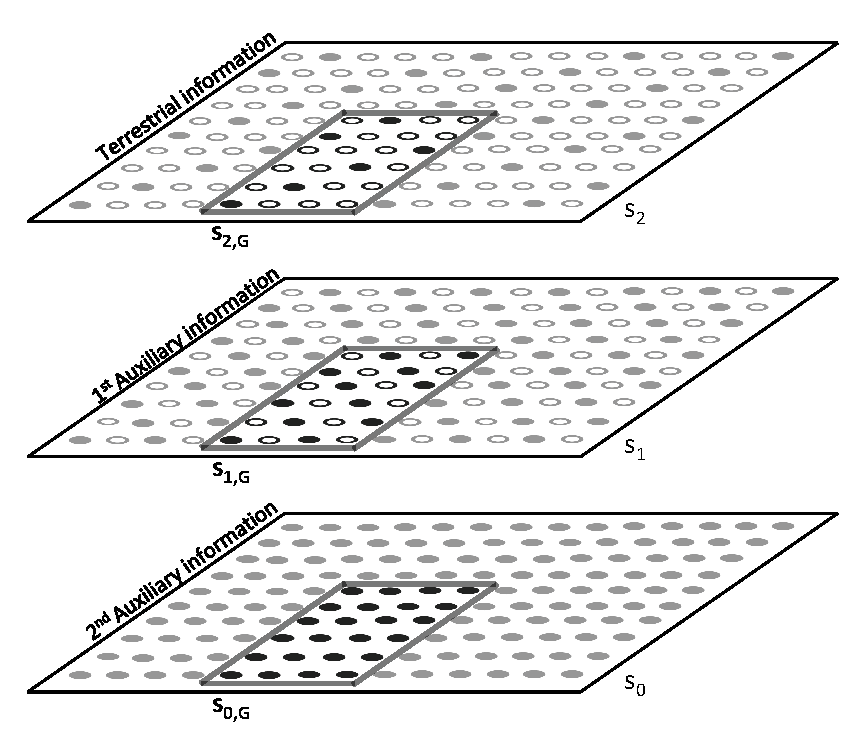
\includegraphics{fig/sae_graphic.eps}}%
		\caption{} \label{fig:concmphase_and_sae_b}
	\end{subfigure}
\caption{\textbf{(a)} Concept of multiphase sampling. The square represents the forest area for which an inventory is being conducted. The points denote the sample locations $x$. Filled points indicate \textit{available} information. \textbf{(b)} Illustration of the Small Area Estimation problem}
\label{fig:concmphase_and_sae}
\end{figure}





% Note that while the auxiliary information is most often provided by remote sensing data, that does not necessarily have to be the case. The auxiliary information can be any information that exhibits a correlation to the local density, i.e. target variable, $Y(x)$.
% 
% e.g. past inventory data \citep{massey2014a}



\subsection{Small Area Estimation}

Explain:
\begin{itemize}
  \item What is the difference between \textit{global} and \textit{small area} estimation?
  \item explain the structure of the package (graphic) and state that we will only concentrate on specific cases ...
\end{itemize}


\begin{figure}[htb]
\centering
\resizebox{1\hsize}{!}{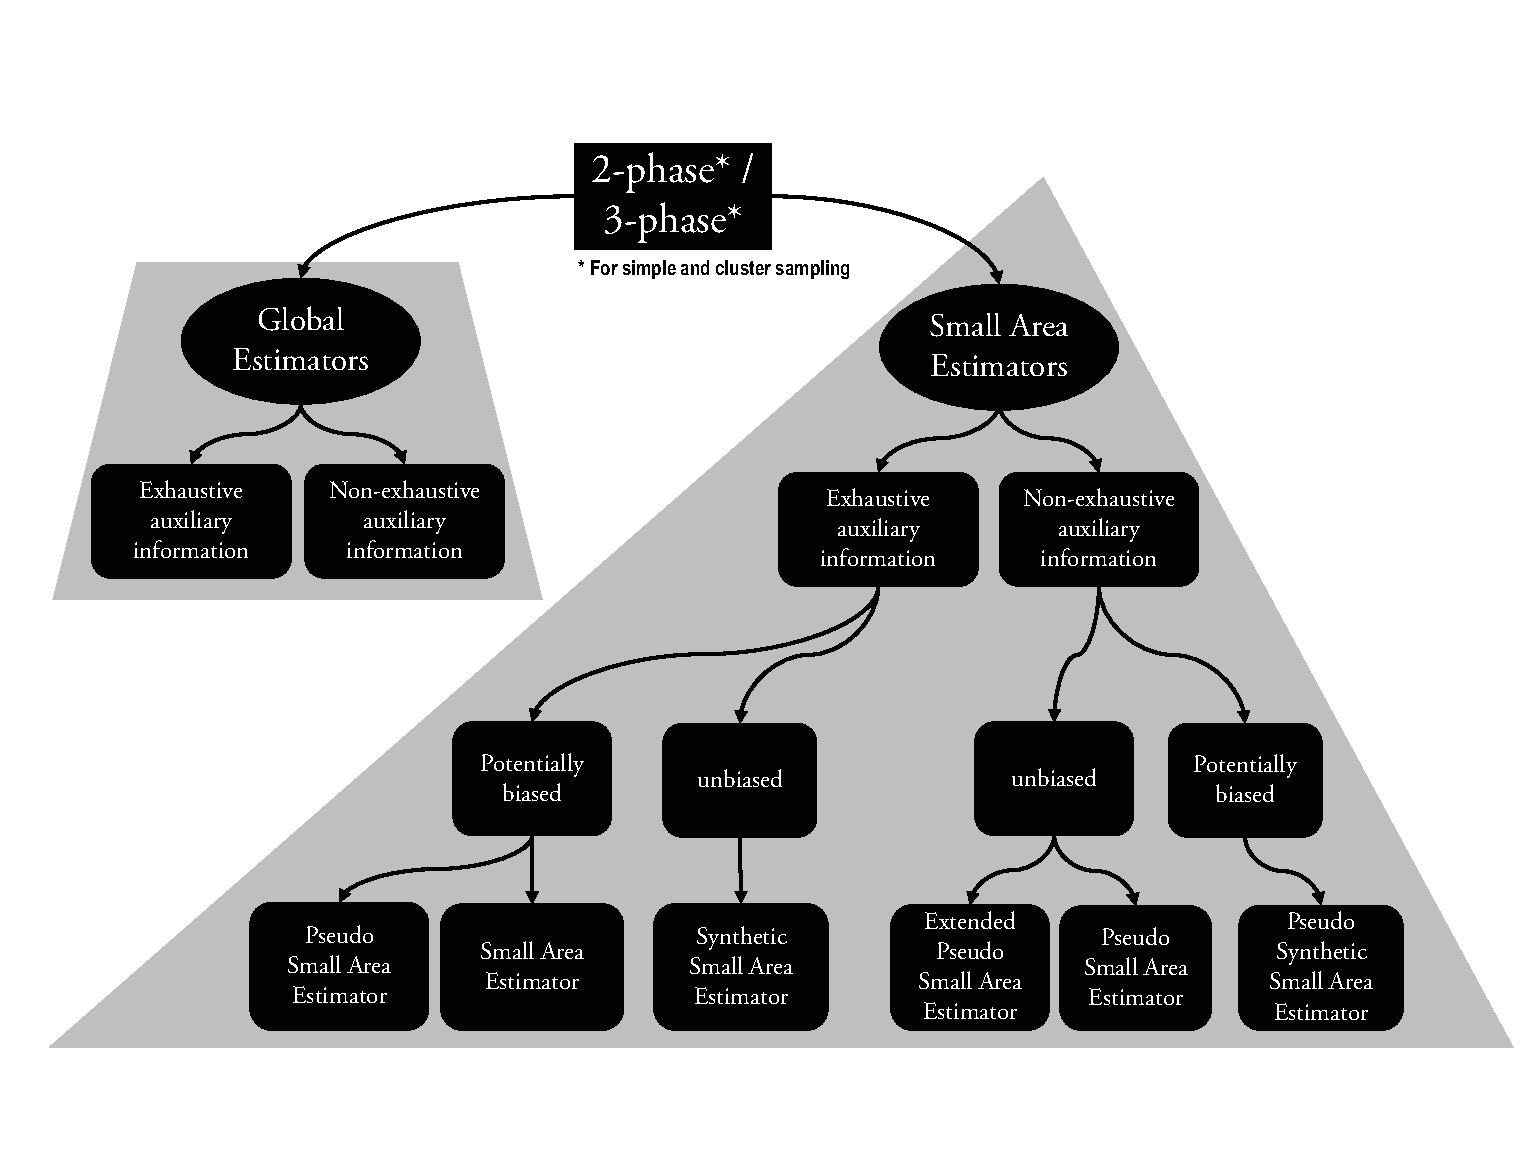
\includegraphics{fig/Package_structure.eps}}
\caption{Structure of the multiphase estimators in the \proglang{R} package \pkg{forestinventory}}
\label{fig:struct_package}
\end{figure}




% NOTES:
% - Pyramide / decision tree Graphik
% - Confidence Interval calculation
% - Analysis of estimations results. a) Visualization functions; b) Gain-analysis
%
% --> explain each point briefly without to much (mathematical) detail



%------------------------------------------------------------------------------------------------%
% ---------------------------------- Estimators and their Application -------------------------- %

%\SweaveInput{rnw/One-Phase Estimators and their Application.Rnw}

% !Rnw root = JStatSoft_forestinventory_master.Rnw

\section[Global Estimators and their Application in R]{Global Estimators and their Application}
\label{sec:globest_and_appl}


% ---------------------------------------------------------------------------- %
\subsection{Double Sampling (Two-Phase) Estimators}

% Note: As the mathematical form of estimators is still quite simple and short, we can here
%       focus on presenting and explaining important 'components' of the estimators, such as Z, C, ...)
% 
% \subsection{Mathematical Background}
% 
% Here, we give the \textbf{mathematical background} of:
% \begin{itemize}
%   \item the classical two-phase estimator, including:
%     \item the external and g-weight variance. Explain the differences and pros for using the g-weight version
%     \item the auxiliary components (Z) and covvar(Z) as well as their use in the point and variance estimator
%   \item the boundary weight adjustment (mathematically: weighted means of Z) --> our extension to the already published stuff
%   \item ...
% \end{itemize}
% 
% 
% 
% \subsubsection{Application}
% 
% Here, we give the \textbf{application} examples:
% \begin{itemize}
%   \item example for non-exhaustive case: use grison dataset
%     \item with boundary adjustments, just mention that this is optional and can be left out, in which case the simple means of Z are used
%   \item example for exhaustive case: use cluster set
% \end{itemize}

\subsubsection{Mathematical Background}

Mention:
\begin{itemize}
  \item What is the difference between model-dependent and design-based? (bias-correction, dont have to believe in model predictions.
  \item explain the structure of the package (graphic) and state that we will only concentrate on specific cases ...
\end{itemize}




The regression coefficients of the OLS regression model are found by solving the sample-based normal equation. In case of \textbf{simple sampling}, the vector of regression coefficients are derived as

\begin{equation}\label{normequ_simple}
  \hat{\pmb{\beta}}_{s_2}&=& \Big(\frac{1}{n_2}\sum_{x\in{s_2}}\pmb{Z}(x)\pmb{Z}^t(x) \Big)^{-1} \Big(\frac{1}{n_2}\sum_{x\in{s_2}}Y(x)\pmb{Z}(x)\Big)
\end{equation}

The design-based variance-covariance matrix of the regression coefficients is then calculated as

\begin{equation}\label{eq:estvarmatrix}
  \hat{\pmb{\Sigma}}_{\hat{\pmb{\beta}}_{s_2}}:=\Big(\frac{1}{n_2}\sum_{x\in{s_2}}\pmb{Z}(x)\pmb{Z}^t(x) \Big)^{-1}
  \Big(\frac{1}{n_2^2}\sum_{x\in{s_2}}\hat{R}^2(x)\pmb{Z}(x)\pmb{Z}(x)^t\Big)
  \Big(\frac{1}{n_2}\sum_{x\in{s_2}}\pmb{Z}(x)\pmb{Z}^t(x) \Big)^{-1} 
\end{equation}

with the empirical residuals, i.e. the regression model residuals, available at all sample location $x \in s_2$ being
\begin{equation}\label{eq:resids}
  \hat{R}(x)=Y(x)-\hat{Y}(x)
\end{equation}

The \textbf{point estimate} for simpe sampling is calculated according to equation \ref{eq:pointest_simple}. Note that this form results under particular case where the regression coefficients are derived using the data from the current inventory (\textbf{internal} regression model). In this case, the mean of the residuals $\frac{1}{n_2}\sum_{x\in{s_2}}R(x)$ is zero by definition and does not have to be added as is necessary for \textbf{external} models. Since in the package \pkg{forestinventory} only allows for internal models, the equation simplifies to

\begin{equation}\label{eq:pointest_simple}
\hat{Y}_{reg}=\hat{\bar{\pmb{Z}}}^t\hat{\pmb{\beta}}_{s_2}
\end{equation}

The estimation precision of the point estimate is specified by the estimated \textbf{design-based variance} as given in equation \ref{eq:gw_var_simple}. Note that this is mathematically identical to the \textbf{g-weight} formulation of the design-based variance given in \citep{mandallaz2016}. The package \pkg{forestinventory} additionally provides the \textbf{external} variance (equation \ref{eq:varexternalsimple}). Note that the external variance neglects the uncertainty in the regression coefficients and is thus usually slightly lower than the design-based variance, where this uncertainty is considered by the variance-covariance matrix of the regression coefficients.

\begin{equation}\label{eq:gw_var_simple}
\hat{\var}(\hat{Y}_{reg})=\hat{\bar{\pmb{Z}}}^t\hat{\pmb{\Sigma}}_{\hat{\pmb{\beta}}_{s_2}}\hat{\bar{\pmb{Z}}}
\end{equation}


\begin{equation}\label{eq:varexternalsimple}
\hat{\var}(\hat{Y}_{reg})=
\frac{1}{n_1}\frac{1}{n_2-1}\sum_{x\in{s_2}}(Y(x)-\bar{Y}_2)^2+
(1-\frac{n_2}{n_1})\frac{1}{n_2}\frac{1}{n_2-1}\sum_{x\in{s_2}}(R(x)-\bar{R})^2
\end{equation}




\subsubsection{Application}





















\subsection{Triple Sampling (Three-Phase) Estimators}


\subsubsection{Mathematical Background}

\subsubsection{Application}



% The psynth estimator:
% 
% \begin{equation}\label{pseudosynth1}
% \hat{Y}_{G,psynth}=\hat{\bar{\pmb{Z}}}_{1,G}^t\hat{\pmb{\beta}}_{s_2}
% =\frac{1}{n_{1,G}}\sum_{x\in{s_{1,G}}}\hat{Y}(x)
% \end{equation}
% 
% \begin{equation}\label{estvarpseudosynth1}
% \hat{\var}(\hat{Y}_{G,psynth}): =
% \hat{\bar{\pmb{Z}}}_{1,G}^t\hat{\pmb{\Sigma}}_{\hat{\pmb{\beta}}_{s_2}}\hat{\bar{\pmb{Z}}}_{1,G}
% + \hat{\pmb{\beta}}_{s_2}^t\hat{\Sigma}_{\hat{\bar{\pmb{Z}}}_{1,G}}\hat{\pmb{\beta}}_{s_2}
% \end{equation}






































% !Rnw root = JStatSoft_forestinventory_master.Rnw

\section[Small Area Estimators and their Application in R]{Small Area Estimators and their Application}
\label{sec:saeest_and_appl}


% ---------------------------------------------------------------------------- %
\subsection{Double Sampling (Two-Phase) Estimators}

% - Merge Mathematical Background and Application
% - Quite Likely, we cannot go through all estimators ...
%   Idea: --> maybe only for non-exhaustive case, and then demonstrate with one example how the exhaustive can be applied in general
%
% - 
%
% - We could give the function call for all cases, but we should only show the output
%   for demonstrating particular things

% Concentrate on subset of estimators to go through the "tree": --> non-exhaustive case
% 1) nex, simple sampling, pseudo extended sae estimator
% 2) nex, simple sampling, pseudo sae estimator
% 3) nex, simple sampling, pseudo synthetic sae estimator --> give reason when to use (if n2G < 5, because ...)
% 
% 4) for the cluster case, show: nex, simple sampling, pseudo extended sae estimator
% 5) for the exhaustive case, show: ex, simple sampling, pseudo extended sae estimator
%    (mention that in cluster case, the cluster means shall be used)
% always use bw-adjustment (?)
%


\subsection{Triple Sampling (Three-Phase) Estimators}













% The psynth estimator:
% 
% \begin{equation}\label{pseudosynth1}
% \hat{Y}_{G,psynth}=\hat{\bar{\pmb{Z}}}_{1,G}^t\hat{\pmb{\beta}}_{s_2}
% =\frac{1}{n_{1,G}}\sum_{x\in{s_{1,G}}}\hat{Y}(x)
% \end{equation}
% 
% \begin{equation}\label{estvarpseudosynth1}
% \hat{\var}(\hat{Y}_{G,psynth}): =
% \hat{\bar{\pmb{Z}}}_{1,G}^t\hat{\pmb{\Sigma}}_{\hat{\pmb{\beta}}_{s_2}}\hat{\bar{\pmb{Z}}}_{1,G}
% + \hat{\pmb{\beta}}_{s_2}^t\hat{\Sigma}_{\hat{\bar{\pmb{Z}}}_{1,G}}\hat{\pmb{\beta}}_{s_2}
% \end{equation}






































% NOTES:
% 1st subsection: Global 2 and 3-phase estimators for simple and cluster sampling
% 2nd subsection: 2- and 3-phase Small Area estiamtors for simple and cluster sampling
%



%------------------------------------------------------------------------------------------------%
% ---------------------------------- Special Cases and Scenarios ------------------------------- %


% NOTES:
% - Error handling and adjustments: Sampling designs not nested
% - Error warning: unbalanced designs and singularities due to missing factor levels in s2-sample (2-phase)
%                   or s2 or/and s1 sample in 3-phase case
% - Error warning: cluster not completely within one small area (--> g-weight variance estimator) +  recommendation



%------------------------------------------------------------------------------------------------%
% ---------------------------------- Calculation of Confidence Intervals ----------------------- %


% NOTES:
% - demonstrate calculation of confidence intervals (give the formulas)



%------------------------------------------------------------------------------------------------%
% ----------------------------- Visualization and Analysis of Estimation Results --------------- %

% NOTES:
% - demonstrate visualization of errors and point-ests + CIs
% - demonstrate a) releff-calculation and gain-analysis



%------------------------------------------------------------------------------------------------%
% ---------------------------------------- Literature ------------------------------------------ %


\bibliography{bib/literature}\newpage\cleardoublepage


% -------------------------------------------------------------------------- %
\end{document}




Hallo. Here comes a first try:

\begin{Schunk}
\begin{Sinput}
R> library(forestinventory)
R> op <- onephase(formula = tvol~1 ,data = grisons,
 +               phase_id =list(phase.col = "phase_id_2p",terrgrid.id = 2))
R> summary(op)
\end{Sinput}
\begin{Soutput}
One-phase estimation
 
Call: 
onephase(formula = tvol ~ 1, data = grisons, phase_id = list(phase.col = "phase_id_2p", 
    terrgrid.id = 2))

Method used:
One-phase estimator
 
Estimation results:
 estimate variance n2
 399.4321 567.2001 67
\end{Soutput}
\end{Schunk}

This was the result






